\chapter{MSM Case Study: Manufacturing Fusion, Sensitivity, and Robustness}
\label{ch:msm}

MSM provides the principal completed external manufacturing evaluation of the
representation, fusion and controlled-robustness questions. Each prediction concerns a
completed cutting interval, with native abnormal cutting as the positive class. Across
the tested target and grouping protocols, the logistic sensor branch ranked these
intervals better than F2, while quality-gate behavior depended on the input condition.
The models were fitted on MSM; this study tests applicability in another domain, not
zero-shot transfer from REASSEMBLE.

\section{Motivation and Research-Question Mapping}
Moving from robotic assembly to milling changes the measurements, observation interval
and target. The question is whether a camera adds useful information beyond the milling
machine's numerical measurements under a new, explicitly grouped assessment.

The study connects the original questions in a controlled sequence. The frozen CNN and
interval statistics test a lightweight representation choice (SQ1); averaging, original
F2 and supplementary quality gates test fusion alternatives (SQ2); controlled input
stresses and explicit absence fallbacks address a bounded part of robustness (SQ3).
Target semantics, grouped assessment, probability quality and the distinction between
software feasibility and predictive value address SQ4. None of these comparisons
establishes early warning before an abnormal cut or transfer without target-domain
fitting.

The pretrained-initialization comparison covered three fixed training seeds and the
specified target, grouping and corruption conditions. An initial development run tested
the implementation on a small sample. Performance estimates came from the subsequent
held-out intervals that met the timing and input-coverage criteria.\ev{MSM experimental
design}{\EvidenceRef{E079}{}}

\section{Dataset, Cutting-Label Semantics, and Domain Challenges}
The source dataset combines laboratory and industrial metal-cutting observations
\citep{Kim2026MSM}. It is a data descriptor, rather than a published
unimodal-versus-fusion benchmark. Its streams have different sampling and refresh rates,
and the smartphone camera is available only in the laboratory material. The evaluated
release is the pinned Kaggle version~2 \citep{MSMKaggle2025}. The retained laboratory
material covers VM20i and VMX30Ui; the industrial VF10 component is outside this visual
comparison because it does not supply the corresponding video. The source overview
describes 56 laboratory experiments. Membership in that inventory is distinct from
admission to the final paired cohort.

Native labels distinguish stable normal cutting, intervention-worthy abnormal cutting,
and stable cutting with a defective tool. Their values are respectively 0, 1 and 2. The
primary binary outcome is label~1 against labels~0 and~2. A negative outcome therefore
means stable cutting under this definition; it does not certify a healthy tool. Expert
annotation uses process behavior, sound and measurements, so the label is an observed
process judgment rather than an independently instrumented future-failure endpoint.
Relabeling every defective-tool interval as abnormal would change the task. The study
instead repeats the pipeline after excluding label~2 and retains that as a distinct
target sensitivity.\ev{MSM target definition}{\EvidenceRef{E074}{}}

Of 2,512 native labeled intervals, 1,895 satisfy the joint video and numerical-input
requirements, including 336 positives. The remaining 617 retain their original labels
and explicit exclusion reasons. One prediction refers to one completed cutting interval.
Neither the whole interval nor its final label is shortened into a prediction horizon
that would establish advance warning.

\subsection{Visibility and Independence Limits}
Milling video can show the machine and process context while coolant, enclosure geometry
and occlusion conceal the tool--workpiece interaction. Successful decoding is therefore
insufficient evidence that the labeled abnormality is optically observable. A visual
classifier may respond to operating context, lighting or experiment-specific appearance
rather than the underlying cutting event. The visual training--assessment
gap quantified in Section~\ref{sec:msm-clean} is compatible with this concern, but does not identify its cause.

The machine stream is also an observation of the process rather than direct,
instantaneous ground truth. Aggregated electrical, load and vibration-related
measurements can describe an interval while smoothing short events. Their timing and
update cadence limit any claim about event onset or control latency. Group identity
creates a further difficulty: experiment folders provide a useful split boundary, but
they are not verified identities for physical tools, workpieces or sessions. These
limits motivate both the technical gates and the stricter grouping sensitivities.\ev{MSM
validation limits}{\EvidenceRef{E075}{}}

\section{Preparation, Timing Alignment, and Cohort Support}
Preparation admits examples only when both modalities meet a fixed input contract.
Acoustic evidence establishes the timing correspondence between video and machine
measurements. The classifier receives video frames and machine-sensor features derived
from fifteen MTConnect channels. The dominant exclusion is lack of validated acoustic timing support, followed by rejected or
insufficient alignment and numerical gaps. These are technical exclusions, not removals
based on model correctness. The exclusion record identifies intervals removed before
modelling. Successful decoding alone does not establish that an anomaly is visible.

\subsection{Video Timing and Interval Correspondence}
The initial alignment pilot estimated video--sensor offsets from matching acoustic
patterns and checked them against withheld acoustic segments. The later laboratory-wide
audit reused the corrected estimator and rejected ambiguous mappings or mappings with
insufficient validation support. The final adapter reuses these accepted offsets without
fitting them against outcome labels. Its convention is video time equal to
sensor time plus the accepted offset, within the region supported by the calibration. A
documented correction matters here: VMX9 uses an offset of $+49.73$~s; the rejected
$+16.04$~s alias is not an interchangeable alternative. Treating the two alignments as
equivalent would change which visual evidence accompanies each native interval.

Cuts use half-open intervals and uncertainty guards. Each admitted interval has sixteen
ordered, distinct native frames with source timestamps and content identities. The
assessment concerns the accepted support, not every point of the original recording. An
accepted offset supplies a defensible correspondence under the recorded calibration; it
does not prove hardware synchronization or eliminate residual timing uncertainty.\ev{MSM
timing and alignment checks}{\EvidenceRef{E075}{}}

\subsection{Visual Coverage and Geometry}
The frozen recipe corrects the source sample aspect ratio of $3{:}8$ and uses
aspect-preserving, centered black letterboxing to $640\times640$. This preserves
geometry instead of stretching narrow process views into a square. Sixteen interval
frames pass through the same CNN, and spatial and temporal means produce one interval
representation. Frame order is retained in provenance but is not learned by the
mean-pooling model.

At least sixteen distinct native frames are required; repeating a short clip to reach
the nominal frame count is not accepted as additional temporal coverage. Later stress
conditions alter actual image content before feature extraction. Neither the common crop
nor a displayed context view is a detector box, a tool annotation, or a verified
abnormal region. The derived galleries support examination of the evidence and errors;
they do not replace independent frame-level annotations.\ev{MSM visual input
contract}{\EvidenceRef{E068}{}}

\subsection{Sensor Coverage and Measurement Interpretation}
The evaluated numerical input comprises fifteen MTConnect channels: power, spindle speed
and load, feed rate, axis loads, and the supplied RMS-related channels. Six
channel-major statistics---mean, population standard deviation, RMS, minimum, maximum
and peak-to-peak---yield ninety values per interval. The channel names and measurement
semantics remain those of the release; they are not recast as a new calibrated force
signal.

Numerical support must contain at least five finite rows, with no gap greater than
$0.5$~s including interval edges. The pipeline neither interpolates an unsupported gap
nor substitutes an accelerometer branch. Means, standard deviations, imputation values
and corruption scales that require population estimation are fitted only within the
appropriate training partition. This prevents the assessment distribution from
influencing the numerical normalization, while leaving the source stream's aggregation
and latency limitations intact.\ev{MSM numerical coverage}{\EvidenceRef{E075}{}}

\subsection{Class Support and Independent Groups}
The primary cohort has 45 nominal experiment groups, 17 containing positives, seven
machine/date proxies and five calendar dates. Every actual fitting, out-of-fold and
assessment partition must contain both classes. Table~\ref{tab:msm-support} records the
positive/total assessment support for all six target/grouping protocols. The folds
within a protocol partition its admitted cohort; the six protocols are sensitivities on
related observations, not six independent datasets.

\begin{table}[htbp]
\caption{Class Counts in the MSM Assessment Folds}\label{tab:msm-support}
\centering\small

\begin{tabular}{lrrr}\hline
Target and grouping & Fold 0 & Fold 1 & Fold 2\\\hline
Primary, experiment &157/567&37/730&142/598\\
Primary, machine/date &38/468&95/664&203/763\\
Primary, calendar date &157/422&99/689&80/784\\
Exclude label 2, experiment &138/712&122/429&76/629\\
Exclude label 2, machine/date &38/447&95/641&203/682\\
Exclude label 2, calendar date &99/645&157/341&80/784\\\hline
\end{tabular}
\displaynote{Each cell gives the number of positive intervals divided by the total
number of intervals. Label~1 is positive.}
\end{table}
\ev{MSM complete split support}{\EvidenceRef{E069}{}}

Experiment and date identifiers serve as proxies for physical independence. Repeated
tool or workpiece use across dates remains unresolved. The additional DOWN-only,
label-2-excluded comparison fails the fixed class-support requirement. The split seeds
and fold counts were fixed, leaving that comparison without an estimate.
Direction-specific held-out summaries are descriptive and cannot isolate a causal effect
of cutting direction.

\begin{figure}[p]
\caption{Paired Camera Frames and Sensor Measurements for an MSM Milling
Interval}\label{fig:msm-example}
\centering
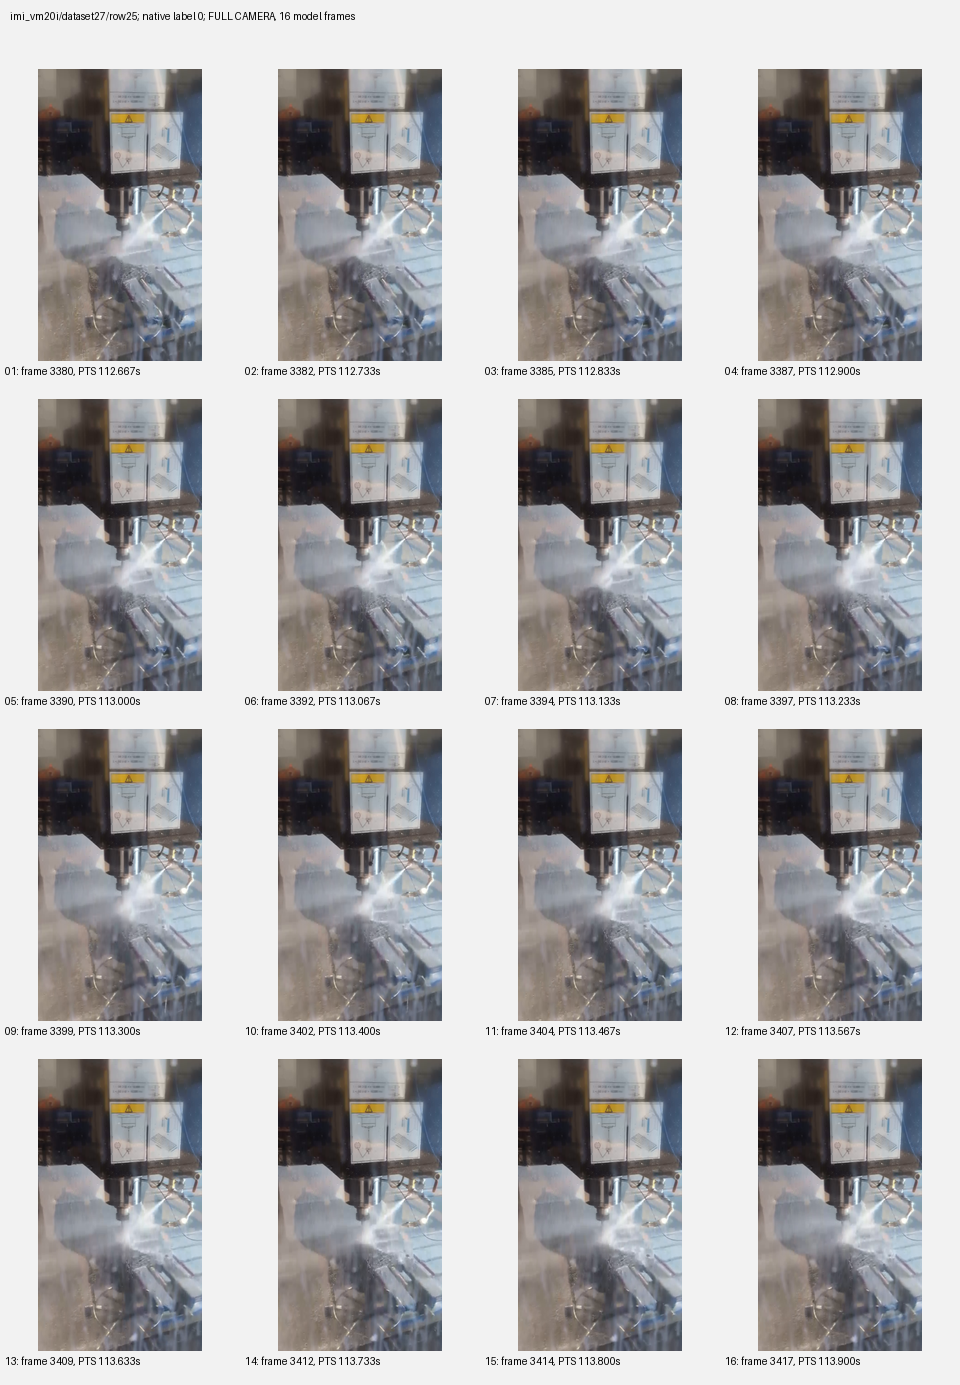
\includegraphics[width=\textwidth,height=.37\textheight,keepaspectratio]{figures/msm_example05_frames.png}\par\vspace{3mm}
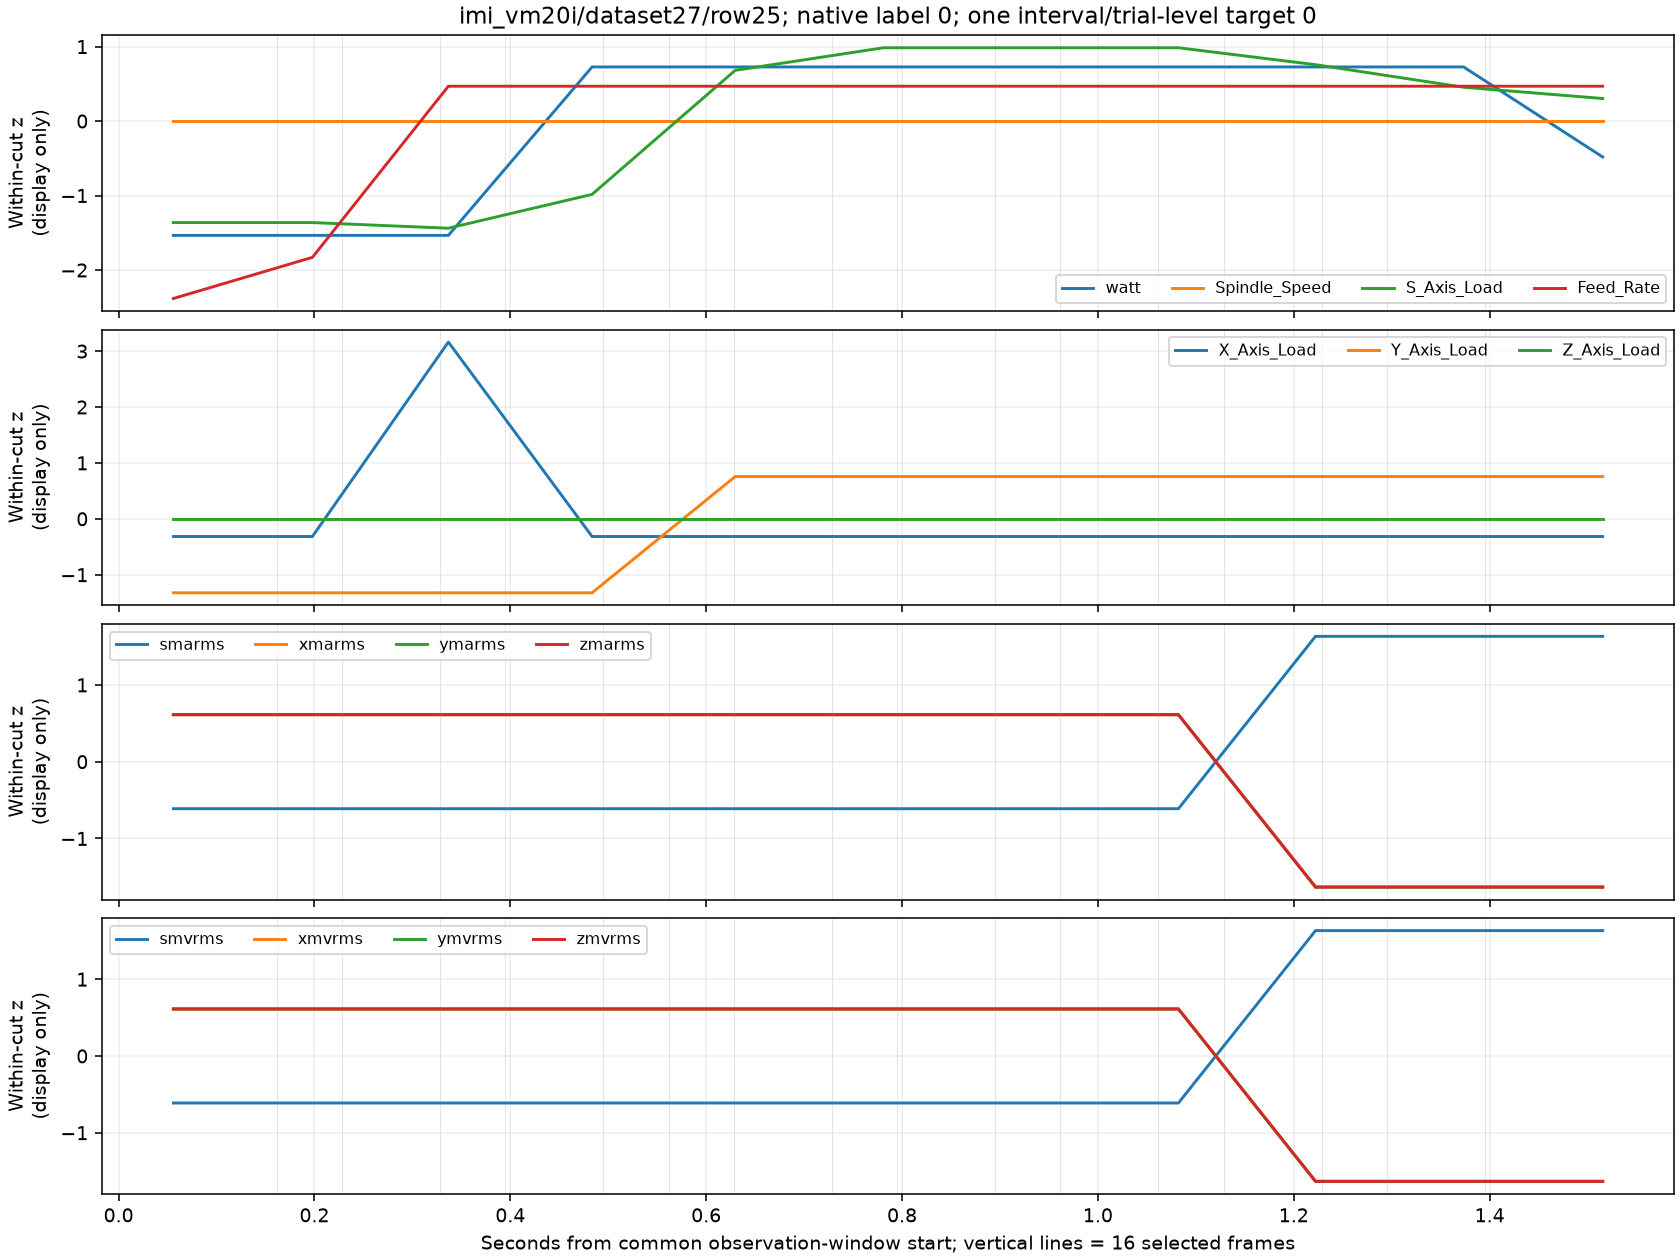
\includegraphics[width=\textwidth,height=.31\textheight,keepaspectratio]{figures/msm_example05_sensor.png}
\displaynote{The 16 frames and time-aligned MTConnect traces cover interval
\texttt{imi\_vm20i/dataset27/row25}, pair P03, at 112.405--113.941~s. The recorded label
is 0 (stable normal). Within-interval $z$ scores scale these curves for display. The
fitted model used training-only normalization and assigned one prediction to the whole
interval.}
\end{figure}
\ev{Illustrative input and identity source}{\EvidenceRef{E071}{}, \EvidenceRef{E072}{},
\EvidenceRef{E073}{data row 5}}
\section{Architecture Reuse, Adaptations, and Evaluation Protocol}
The pretrained condition (P) used the ResNet18-vd CNN backbone inside the RT-DETR-R18vd
checkpoint \citep{Zhao2024RTDETR}. The extractor stopped at the CNN feature maps, before
the hybrid Transformer encoder, detection decoder, and box heads. Spatial means from the
last three maps yielded 896 features per frame. Averaging across sixteen frames gave one
vector per cutting interval. With the backbone frozen, a newly fitted
$896\rightarrow128\rightarrow1$ head with ReLU and dropout~0.1 supplied the target
prediction. It had 114,945 trainable parameters.

The numerical branch is a fresh balanced L2 logistic regression on the ninety
statistics, with $C=1$. A separately fitted histogram gradient boosting model provides
the stronger sensor control. It is essential to keep that control separate: F2 consumes
the logistic branch, not the HGB predictions. Averaging combines the two branch
probabilities without a fitted fusion parameter. Original F2 is a newly fitted
unweighted L2 logistic model on visual and sensor probabilities generated out of fold.
No source failure head, scaler, calibrator or fusion coefficient is transferred.\ev{MSM
executed composition}{\EvidenceRef{E077}{}}

The clean and augmented quality gates are additional comparisons. They reuse a small
softmax gate over branch logits, with label-free image-quality summaries, numerical
variability, missing-channel fractions and availability flags. These summaries may
encode process context as well as degradation. A changing allocation therefore is not a
calibrated estimate of modality reliability. This matters because a reliability-aware
fusion argument requires a quality proxy that actually predicts error, rather than a
proxy that merely changes with the input \citep{Zhang2023QMF}. QG-clean uses clean OOF
views. QG-aug sees clean views plus seven predefined lowest-severity corruptions, while
F2-aug is the exposure-matched static control. Clean fitting, corruption exposure and
quality conditioning remain separate interventions.

R denotes a different question: initialization from a specifically completed
REASSEMBLE-learned CNN. The exact canonical source required by MSM's gate was
unavailable in the inspected evaluation, so that condition remains unmeasured. This does
not contradict the P completion or the later, differently specified ViFailback donor
study. Architecture reuse, generic pretraining and transfer of task-learned weights
retain separate provenance.

\subsection{Implementation Checks and Bounded Development Run}
The bounded development exercise was an engineering check: its two-epoch,
at-most-24-interval design restricted head updates and CNN frame forwards and prohibited
outer-assessment predictions. It could expose shape, gradient, memory or reload errors,
but could not estimate generalization. Generalization was assessed in the subsequent
evaluation on held-out intervals.

The saved implementation audit checks planned cases, source identities, native
assessment units, model budgets and checkpoint reloads. It also refits the fixed F2
estimator from saved clean OOF probabilities and reports zero coefficient discrepancy.
The CNN cache check reports maximum difference zero on an outer-training-only example.
These support consistency of the saved procedure and its outputs. Their scope is
narrower than reproduction of stochastic training: exact reload and metric recomputation
cannot alone certify that every training step would recur in another environment.\ev{MSM
implementation and reproduction scope}{\EvidenceRef{E078}{}}

\subsection{Evaluation Protocol and Conditions Without Estimates}
The completed matrix uses three outer and two inner StratifiedGroupKFold partitions,
fixed split seeds and training seeds 42, 123 and 20261023. Inner fits produce branch OOF
probabilities for learned fusion; outer assessments remain excluded from fitting. The
six target/grouping protocols yield 54 completed case records. The 54 cases include
different folds and seeds from overlapping protocols.

The main visual head runs for ten fixed epochs and the gate for forty. The assessment
uses a fixed threshold of 0.5, with no assessment-selected epoch or fitted primary
calibrator. The definitions in Section~\ref{sec:ch4-metrics} apply: AP is average precision,
not trapezoidal PR area, and F2 names the stacker. Each seed's disjoint outer predictions
are pooled before AP is computed; the three seed-specific APs are then summarized.
These are not mean-fold APs.

Conditions with a missing source checkpoint, inadequate class support or insufficient
temporal coverage yielded no estimate. The results below cover the conditions that met
the original criteria.\ev{MSM fixed evaluation protocol}{\EvidenceRef{E070}{}}

\section{Investigation A: Clean Unimodal and Fusion Comparison}
\label{sec:msm-clean}
On intact inputs, F2 had lower AP than its logistic sensor component at all three seeds.
The mean paired difference was $-0.0717$ (Table~\ref{tab:msm-clean}). F2 ranked
abnormal intervals more accurately than the visual branch or equal averaging. Sensor HGB
had the highest mean AP of the models compared.

\begin{table}[htbp]
\caption{MSM Prediction Performance With Intact Inputs}\label{tab:msm-clean}
\centering\small

\begin{tabular}{lrr}\hline Model&Mean AP&Seed SD\\\hline
Visual&0.2989&0.0109\\
Sensor logistic&0.8286&0.0000\\
Sensor HGB&0.9013&0.0000\\
Averaging&0.7356&0.0159\\
F2&0.7569&0.0111\\
F2-aug&0.7602&0.0098\\
QG-clean&0.8374&0.0134\\
QG-aug&0.8265&0.0162\\\hline
\end{tabular}
\displaynote{Entries summarize pooled average precision across three fixed seeds as the
mean and sample standard deviation.}
\end{table}
\ev{MSM primary results}{\EvidenceRef{E076}{}}

The visual training diagnostic averaged AP 0.9807 across the nine outer fits
(three folds by three seeds; range 0.9634--0.9994), compared with mean seed-specific
pooled held-out AP 0.2989. The training score is an in-sample mean on overlapping training
sets, not a second pooled assessment score. These predictions did not enter F2.
The gap is consistent with overfitting or acquisition shift, but does not isolate
visibility, alignment or representation quality as its cause.\ev{Visual training and
held-out diagnostics}{\EvidenceRef{E137}{}}

\section{Investigation B: Target-Definition and Grouping Sensitivities}
Logistic sensing had higher mean AP than F2 in all six prespecified protocols. Excluding
label~2 and grouping by calendar date gave 0.5218 for F2 and 0.8917 for logistic
sensing. That sensitivity analysis changes the target. Under the primary definition,
pooled prevalence was $336/1{,}895=0.1773$ and outer-fold prevalences ranged from
approximately 0.051 to 0.277. The fold-specific training-prior baseline had pooled AP
0.1454 because the fitted prior could vary across folds.


\begin{table}[htbp]
\caption{MSM Clean Performance Across All Six Protocols}\label{tab:msm-sensitivity}
\centering\small
\setlength{\tabcolsep}{4pt}
\begin{tabular}{lrrrrr}\toprule
Target and grouping & Vision & Sensor LR & HGB & F2 & QG-clean\\\midrule
Primary, experiment & 0.2989 & 0.8286 & 0.9013 & 0.7569 & 0.8374\\
Primary, machine/date & 0.5359 & 0.8922 & 0.8250 & 0.7389 & 0.8715\\
Primary, calendar date & 0.5444 & 0.8859 & 0.8386 & 0.8196 & 0.8521\\
Exclude 2, experiment & 0.3164 & 0.9403 & 0.8965 & 0.8235 & 0.9308\\
Exclude 2, machine/date & 0.3396 & 0.9265 & 0.9098 & 0.8562 & 0.7372\\
Exclude 2, calendar date & 0.4009 & 0.8917 & 0.9062 & 0.5218 & 0.6757\\
\bottomrule\end{tabular}
\displaynote{Mean of three seed-specific pooled abnormal-cutting APs. Primary protocols
use 1,895 intervals; label-2 exclusion leaves 1,770. All retain 336 positives.
Protocols reuse observations and change the fitting/assessment groups; they are
sensitivity analyses, not independent replications.}
\end{table}
\ev{All-protocol saved results}{\EvidenceRef{E135}{}, \EvidenceRef{E081}{}}

The sensor-reference ranking also depends on the protocol: logistic sensing has higher
mean AP than HGB in four of the six comparisons, while HGB leads in the primary
experiment-grouped comparison. The stronger sensor model is therefore not the same
across all target definitions and grouping choices.

For the primary experiment-grouped protocol, the mean F2-minus-logistic AP difference
of $-0.0717$ has a paired 95\% bootstrap interval of $[-0.1605,+0.0031]$ when
resampling 45 experiment folders, and $[-0.1004,-0.0515]$ when resampling five calendar
dates. These intervals use the same held-out predictions with different resampling
units. The folder interval includes zero; the date interval is wholly negative. Across
the six protocols, all observed mean differences favor logistic sensing, and five of
the six folder-bootstrap intervals exclude zero. Both bootstrap schemes hold fits and
split assignments fixed and cannot account for unidentified equipment reuse.

QG-clean averaged $0.0088$ AP above logistic sensing, with one negative seed and a
calendar-date bootstrap interval of $[-0.0971,0.0564]$. The interval admits gains and
losses and leaves equivalence unresolved.\ev{Milling results and paired bootstrap
units}{\EvidenceRef{E081}{}, \EvidenceRef{E144}{}}

\section{Investigation C: Input Degradation, Quality Gates, and Fallback}
Table~\ref{tab:msm-robustness} covers the strongest declared severity of all seven
corruption families. F2-aug and QG-aug have matched augmentation exposure; this control
separates quality conditioning from additional corruption training.

At the highest sensor-noise level, QG-aug reached 0.2986 mean AP, close to intact
vision at 0.2989. F2 reached 0.2069 and noisy sensor HGB reached 0.6062. Under the
strongest image blur, QG-aug achieved 0.6828, below F2 at 0.7714 and intact logistic
sensing at 0.8286. The comparison therefore depends on which stream deteriorates and
which predictor remains available. The tests also covered brightness and contrast
changes, occlusion, frame omission, zeroed channels and explicitly missing channels.


\begin{table}[htbp]
\caption{MSM High-Severity Corruption and Known Absence}\label{tab:msm-robustness}
\centering\small\setlength{\tabcolsep}{4pt}
\begin{tabular}{lrrrrr}\toprule
Condition & Intact & F2 & F2-aug & QG-aug & HGB\\\midrule
Blur ($\sigma=4$) & 0.8286 & 0.7714 & 0.7712 & 0.6828 & 0.9013\\
Brightness/contrast (0.2) & 0.8286 & 0.7700 & 0.7688 & 0.6787 & 0.9013\\
Occlusion (40\%) & 0.8286 & 0.7708 & 0.7709 & 0.8332 & 0.9013\\
Frame omission (12/16) & 0.8286 & 0.7604 & 0.7654 & 0.8331 & 0.9013\\
Sensor noise ($1\,\mathrm{SD}$) & 0.2989 & 0.2069 & 0.2062 & 0.2986 & 0.6062\\
Zeroed channels (50\%) & 0.2989 & 0.4198 & 0.4188 & 0.4754 & 0.6466\\
Missing channels (50\%) & 0.2989 & 0.4477 & 0.4469 & 0.5115 & 0.5460\\
Vision absent & 0.8286 & 0.8286 & 0.8286 & 0.8286 & 0.9013\\
Sensors absent & 0.2989 & 0.2989 & 0.2989 & 0.2989 & --\\
\bottomrule\end{tabular}
\displaynote{Mean seed-specific pooled AP on the primary cohort. Intact denotes
logistic sensing for visual faults and vision for sensor faults. HGB receives the
same sensor condition; it is unavailable when all sensors are absent. Known absence
uses the programmed survivor route. Intermediate severities remain in the saved
robustness report (E080).}
\end{table}
\ev{All seven stress families}{\EvidenceRef{E136}{}, \EvidenceRef{E080}{}}

Whole-modality absence invokes a separately programmed surviving-branch fallback:
0.8286 AP without vision and 0.2989 without sensors. Equal fallback scores across
fusion methods are imposed behavior, not adaptive recovery learned from data.
Differences in augmentation exposure between a gate and its static control would
confound the effect of quality conditioning.\ev{MSM input perturbation and fallback
results}{\EvidenceRef{E080}{}}

\section{Metric Trade-offs, Limitations, and Transition to ViFailback}
For seed~42, F2 had lower AP than logistic sensing but a lower Brier score (0.0561
versus 0.0617) and higher F1 score (0.8204 versus 0.8113). QG-clean had higher AP than
F2, a worse Brier score of 0.0644 and a lower F1 score of 0.7864. Thus the ranking
comparison favored logistic sensing, whereas probability error and fixed-threshold
decisions favored F2 for this seed. The relative performance of the gates depended on
the input condition.

The logistic sensor model uses balanced class weights and no fitted primary calibrator,
whereas F2 is unweighted and fits an intercept and two coefficients to group-OOF branch
probabilities. These different fitting objectives and probability mappings can affect
probability error and ranking differently. They offer a plausible explanation for the
AP--Brier trade-off, but this comparison does not isolate class weighting, the added
visual input or the fitted mapping as its cause.\ev{MSM seed-42 scores and fitting
definitions}{\EvidenceRef{E136}{}, \EvidenceRef{E068}{}, \EvidenceRef{E149}{},
\EvidenceRef{E150}{}}

The visual model ranked held-out intervals poorly despite a much stronger training
result. Inadequate features, limited event visibility, residual alignment error and
experiment-specific appearance could each contribute. Independent annotations of event
visibility and a matched representation comparison on the same groups would help
distinguish these explanations.

MSM therefore supplies a completed external comparison of representations, fusion,
target/grouping sensitivity and controlled robustness. Its unavailable R condition
leaves learned-weight transfer unanswered. Chapter~\ref{ch:vifailback} addresses that
separate question with a specified REASSEMBLE donor and task-disjoint robotic episodes,
while retaining its narrower adaptation coverage and unexecuted corruption study.
